\documentclass[tikz, border=8pt]{standalone}
\usepackage{tikz}
\usetikzlibrary{calc}
\definecolor{bukubiru}{HTML}{2E5E8C}
\definecolor{bukukuning}{HTML}{F7B538}
\definecolor{navy}{HTML}{14213D}

% Satu gambar buku: persegi tegak dengan punggung di kiri
% dan dua garis putih sebagai baris teks.
\tikzset{
  pics/buku/.style={
    code={
      \draw[fill=bukubiru, draw=navy, thick] (0,0) rectangle (0.8,1);
      \draw[navy, thick] (0.18,0) -- (0.18,1);
      \draw[white, thick] (0.32,0.72) -- (0.66,0.72);
      \draw[white, thick] (0.32,0.45) -- (0.66,0.45);
    }
  }
}

\begin{document}

% ---------------------------------------------------------------
% Gambar 1: Piktogram utama.
% Buku yang dibaca kelas VIII.A, Januari--Mei.
% Legenda: 1 gambar buku = 2 buku.
% Januari 10, Februari 16, Maret 14, April 8, Mei 12.
% ---------------------------------------------------------------
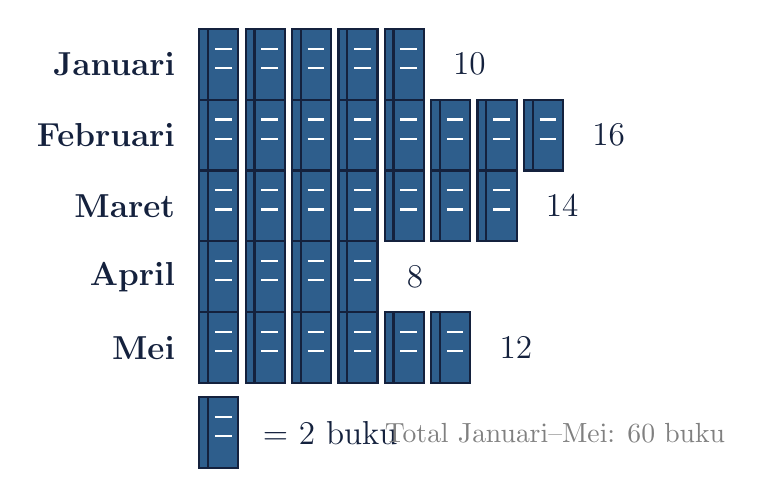
\begin{tikzpicture}[x=0.62cm, y=0.9cm]
  \foreach \bulan/\jumlah/\total/\y in
    {Januari/5/10/5, Februari/8/16/4, Maret/7/14/3,
     April/4/8/2, Mei/6/12/1} {
    \node[anchor=east, font=\large\bfseries, navy] at (-0.3,\y) {\bulan};
    \foreach \i in {1,...,\jumlah} {
      \pic at ({(\i-1)*0.95}, \y-0.5) {buku};
    }
    \node[anchor=west, font=\large, navy] at ({\jumlah*0.95+0.25}, \y) {\total};
  }
  % Legenda di bawah diagram
  \pic at (0,-0.7) {buku};
  \node[anchor=west, font=\large, navy] at (1.1,-0.2) {= 2 buku};
  \node[anchor=west, font=\normalsize, gray] at (3.6,-0.2)
    {Total Januari--Mei: 60 buku};
\end{tikzpicture}

% ---------------------------------------------------------------
% Gambar 2: Setengah gambar untuk bilangan ganjil.
% Juni: 15 buku = 7 gambar penuh + 1 setengah gambar.
% Setengah kanan ditutup clip; garis putus-putus menandai
% bagian yang sengaja tidak digambar.
% ---------------------------------------------------------------
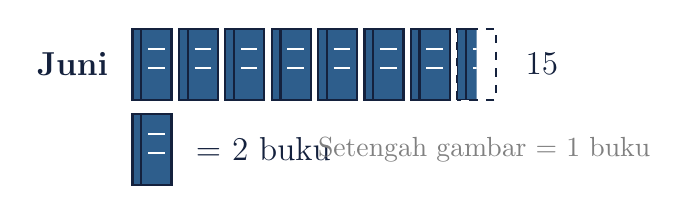
\begin{tikzpicture}[x=0.62cm, y=0.9cm]
  \node[anchor=east, font=\large\bfseries, navy] at (-0.3,1) {Juni};
  \foreach \i in {1,...,7} {
    \pic at ({(\i-1)*0.95}, 0.5) {buku};
  }
  % Setengah buku ke-8
  \begin{scope}
    \clip ({7*0.95},0.5) rectangle ({7*0.95+0.4},1.5);
    \pic at ({7*0.95}, 0.5) {buku};
  \end{scope}
  \draw[navy, dashed, thick]
    ({7*0.95},0.5) rectangle ({7*0.95+0.8},1.5);
  \node[anchor=west, font=\large, navy] at ({8*0.95+0.25}, 1) {15};
  % Legenda
  \pic at (0,-0.7) {buku};
  \node[anchor=west, font=\large, navy] at (1.1,-0.2) {= 2 buku};
  \node[anchor=west, font=\normalsize, gray] at (3.6,-0.2)
    {Setengah gambar = 1 buku};
\end{tikzpicture}

\end{document}
